% Tipo de documento
\documentclass[12pt,a4paper]{article}

% Pacotes
%\usepackage{showlabels}
\usepackage{latexsym}
\usepackage{amsfonts}
\usepackage{amsmath}
\usepackage{amscd}
\usepackage[brazil]{babel}
\usepackage[utf8]{inputenc}
\usepackage[pdftex]{graphicx} 

% Paginação
%\textwidth 15.0cm                    % Largura
%\textheight 22.0cm                   % Altura
%\addtolength{\oddsidemargin}{0.0cm}  % Margem esquerda (impar)
%\addtolength{\evensidemargin}{0.0cm} % Margem esquerda (par)
%\addtolength{\topmargin}{0.0cm}      % Margem superior

% Estilo dos parágrafos
\sloppy                              % Mais flexível
\setlength{\jot}{08pt}               % Distância entre linhas do eqnarray
\setlength{\parskip}{1ex}            % Distância entre parágrafos
\renewcommand{\baselinestretch}{1.0} % Distância entre linhas

% Comandos customizados
\newcommand{\vet}{\mathbf}                                   % vetor
\newcommand{\ie}{\emph{i.e.}}                                % isto é
\newcommand{\prodint}[2]{\left\langle #1 , #2 \right\rangle} % produto interno
\newcommand{\Fullbox}{{\rule{2.0mm}{2.0mm}}}                 % caixa cheia
\newcommand{\EOS}{\hfill\Box\vspace{-0.2cm}}                 % fim de enunciado
\newcommand{\EOP}{\hfill\Fullbox\vspace{0.2cm}}              % fim de prova
\newcommand{\eps}{\varepsilon}                               % epsilon
\newcommand{\defi}{\: := \: }                                % definição
\newcommand{\del}{\partial}                                  % derivada parcial
\newcommand{\hsp}{\hspace{0.5cm}}                            % espaco horizontal para fórmulas
\newcommand{\vsp}{\vspace{0.1cm}}                            % espaco vertical para fórmulas
\newcommand{\ev}{\, ,}                                       % espaco e virgula
\newcommand{\ep}{\, .}                                       % espaco e ponto
\newcommand{\eg}{\emph{e.g.,}}                               % por exemplo

% Fontes caligráficas
\newcommand{\calA}{\mathcal{A}} 
\newcommand{\calC}{\mathcal{C}}
\newcommand{\calR}{\mathcal{R}}                             

% Contagem de equações por seção
\renewcommand{\theequation}{\thesection.\arabic{equation}}

% Contagem de figuras por seção
\renewcommand{\thefigure}{\thesection.\arabic{figure}}

% Contagem de tabelas por seção
\renewcommand{\thetable}{\thesection.\arabic{table}}

% Zerar as contagem em cada seção
\newcommand{\zerar}{\setcounter{equation}{0}\setcounter{figure}{0}\setcounter{table}{0}}

% Operadores
\DeclareMathOperator{\sen}{sen}
\DeclareMathOperator{\tg}{tg}
\DeclareMathOperator{\cotg}{cotg}
\DeclareMathOperator{\im}{im}
\DeclareMathOperator{\arctg}{arctg}
\DeclareMathOperator{\diag}{diag}
\DeclareMathOperator{\sgn}{sgn}
\DeclareMathOperator{\tr}{tr}

% Conjunto de números
\newcommand{\Z}{\mathbb{Z}}
\newcommand{\C}{\mathbb{C}}
\newcommand{\N}{\mathbb{N}}
\newcommand{\Q}{\mathbb{Q}}
\newcommand{\R}{\mathbb{R}}

%%%%%%%%%%%%%%%%%%%%%%%%%%%%%%%%%%%%%%%%%%%%%%%%%%%%%%%%%%%%%%%%%%%%%%%%%%%%%%%%%%%%%%%%%%%%%%%%%%%%

\begin{document}

\title{\bf Otimização de Escalas de Tripulantes em Companhias Aéreas}
\author{Daniel Augusto Cortez \\ Lucas Rodrigues Colucci \\ Renato Lerac Corrêa de Sá}
\date{\today}

\maketitle

\begin{abstract}
	Fornecemos as motivações e a formulação do problema de otimização de escalas de tripulantes em 
	companhias aéreas. O problema é normalmente decomposto em dois subproblemas resolvidos 
	sequencialmente: determinação de viagens e determinação de escalas. Um modelo de programação 
	linear inteiro é apresentado para resolver cada um.
\end{abstract}

\thispagestyle{empty}

\newpage 

\tableofcontents

\newpage

%%%%%%%%%%%%%%%%%%%%%%%%%%%%%%%%%%%%%%%%%%%%%%%%%%%%%%%%%%%%%%%%%%%%%%%%%%%%%%%%%%%%%%%%%%%%%%%%%%%%

\zerar
\section{Introdução}
\label{sec:introducao}

Métodos de otimização no planejamento das operações de uma empresa aérea têm sido aplicados a várias
décadas~\cite{yu}. Tal planejamento envolve diversos problemas que normalmente são resolvidos de
forma separada e seqüencial devido ao tamanho e a complexibilidade de cada problema individual,
embora eles estejam intimamente relacionados~\cite{barnhart03} (veja Figura~\ref{fig:planejamento}).

Primeiro, resolve-se o problema da \emph{malha de voos}, que consiste em determinar todos os trechos
a serem voados pela empresa num determinado período de tempo. O planejamento é basicamente feito em
termos de demanda de mercado.

Segundo, trata-se do problema da \emph{atribuição de frotas}. Nele, determina-se qual o tipo de
aeronave (tal como Boeing 737, Boeing 767, Airbus 320, etc) deve ser atribuído para efetuar cada
trecho da malha de voos. O objetivo é maximizar os lucros de venda, em função da demanda prevista e
do custo de se operar determinada frota em determinado trecho, sujeito à restrição de que todos os
voos da malha sejam cobertos com as frotas disponíveis.

Terceiro, considera-se o problema do \emph{roteamento de aeronaves}, que envolve a escolha das
aeronaves de uma frota que vão realizar determinados voos de forma que cada aeronave passe um tempo
adequado em aeroportos específicos com a finalidade de serem revisadas pela manutenção. O objetivo é
maximizar os lucros, respeitando ainda a restrição de que todos os voos da frota sejam cobertos.

Finalmente, o problema de \emph{escalonamento de tripulantes} é resolvido. Tal problema foi um dos
primeiros a receber atenção significativa por parte da comunidade de pesquisa
operacional~\cite{arabeyre69}, sendo ainda um dos mais estudados. Isso porque, no transporte aéreo,
os custos com a tripulação representam a segunda maior parcela dos custos operacionais da empresa,
perdendo apenas para os custos com combustível. Para se ter uma ideia, o custo total com tripulação
excede 1,3 bilhões de dólares todo ano na Americam Airlines~\cite{anbil91a}. Hoje em dia, a
otimização no planejamento de escalas representa economia de cerca de 50 milhões de dólares anuais
para uma companhia de grande porte~\cite{barnhart03}.

\begin{figure}[htbp]
	\begin{center}
		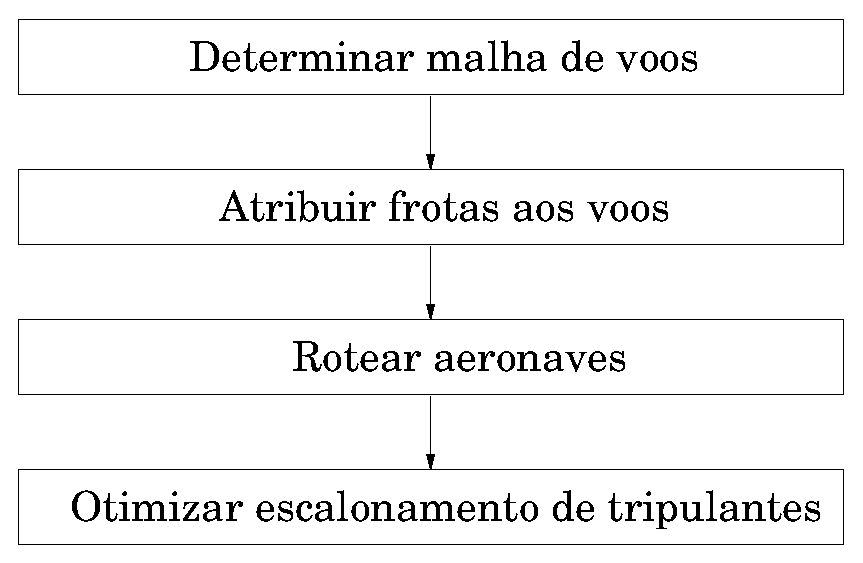
\includegraphics[scale=0.5]{fig/planejamento.eps}
		\caption{Sequência de problemas resolvidos no planejamento de operações de uma empresa aérea.}
		\label{fig:planejamento}
	\end{center}
\end{figure}

De forma geral, escalonamento de tripulantes pode ser definido como o problema de se atribuir um
grupo de trabalhadores (uma tripulação) para realizar um conjunto de atividades. No contexto da
aviação, cada tripulante (comandante, co-piloto, comissário, etc) deve ser designado para realizar
um determinado voo da empresa. Tal designação deve ser feita respeitando-se uma série de restrições
impostas pelas agências reguladoras da aviação, bem como regras de regulamentação trabalhista,
restrições operacionais impostas pela própria empresa e acordos trabalhistas entre empregado e
empregador. Dado o grande número de variáveis e restrições envolvidas, assim como a possibilidade de
grandes ganhos econômicos, o problema torna-se bastante interessante, tanto do ponto de vista da
indústria, quanto acadêmico.

Os objetivos deste primeiro trabalho é dar uma descrição mais precisa do problema de escalonamento
de tripulantes, fornecer uma formulação precisa e discutir brevemente algumas técnicas de solução já
aplicadas para resolução do mesmo.

%%%%%%%%%%%%%%%%%%%%%%%%%%%%%%%%%%%%%%%%%%%%%%%%%%%%%%%%%%%%%%%%%%%%%%%%%%%%%%%%%%%%%%%%%%%%%%%%%%%%

\subsection{Definições e Nomenclaturas}
\label{sec:definicoes}

Antes que possamos apresentar e explorar a estrutura do problema com mais detalhes, faz-se
necessário a introdução de algumas definições e nomenclaturas normalmente utilizadas, as quais serão
amplamente utilizadas neste trabalho.

\begin{itemize}
	\item {\bf Etapa:} é um voo único sem paradas, também chamado de {\bf perna}, {\bf trecho} ou {\bf 
	segmento de voo}.
	\item {\bf Jornada:} conjunto de uma ou mais etapas seqüenciais, também chamado de {\bf jornada 
	de trabalho}. 
	\item {\bf Tempo Mínimo de Conexão:} menor intervalo possível de tempo entre duas etapas 
	consecutivas em uma jornada.
	\item {\bf Tempo Máximo de Conexão:} maior intervalo possível de tempo entre duas etapas 
	consecutivos em uma jornada.
	\item {\bf Tempo de Briefing:} tempo mínimo que antecede o início da primeira etapa de uma
	jornada, necessário para o {\it briefing} da tripulação.
	\item {\bf Tempo de Debriefing:} tempo mínimo que sucede o término da último etapa de uma jornada,
	necessário para o {\it debriefing} da tripulação.
	\item {\bf Início da Jornada:} horário em que a tripulação deve se apresentar para o inicio de
	uma jornada. Corresponde ao horário da decolagem da primeira etapa menos o tempo de briefing. 
	Também chamado de {\bf checkin}.
	\item {\bf Término da Jornada:} horário em que a tripulação encerra suas atividade em uma 
	jornada. Corresponde ao horário de pouso da última etapa mais o tempo de debriefing.
	Também chamado de {\bf checkout}.
	\item {\bf Base Contratual:} cidade onde uma dado tripulante está domiciliado, também chamada 
	simplesmente de {\bf base}.
	\item {\bf Viagem:} conjunto de jornadas de trabalho, com a primeiro etapa da primeira jornada e
	a última etapa da última jornada começando e terminando na mesma base contratual. 
	Uma viagem também é chamada de {\bf pairing}, ou {\bf rotação}.
	\item {\bf Descanso:} intervalo mínimo de tempo ininterrupto de repouso após uma jornada.
	\item {\bf Pernoite:} intervalo de tempo separando duas jornadas consecutivas de uma viagem.
	\item {\bf Reserva:} período de tempo em que o tripulante permanece, por determinação do 
	empregador, em local de trabalho à sua disposição.
	\item {\bf Sobreaviso:} período de tempo não excedente a 12 horas, em que o tripulante permanece 
	em local de sua escolha, à disposição do empregador, devendo apresentar-se em até 90 minutos após 
	receber comunicação para o início de nova tarefa.
	\item {\bf Folga:} período de tempo não inferior a 24 horas consecutivas em que o tripulante, em 
	sua base contratual, sem prejuízo de remuneração, está desobrigado de qualquer atividade
	relacionada com seu trabalho.
	\item {\bf Escala:} conjunto de viagens, reservas, sobreavisos, folgas e deveres extra-voo
	(cursos, treinamentos em simulador, férias, etc), expandindo um determinado horizonte de tempo, 
	que definem as atividades de um tripulante. 
\end{itemize}

A Figura~\ref{fig:viagem} apresenta o exemplo de uma viagem que ilustra alguns dos conceitos
expostos acima. As etapas na figura estão representadas pelos retângulos mais internos. São
indicados os aeroportos de origem e destino, e os horários de decolagem e pouso. As
jornadas são indicadas pelos retângulos pontilhados reúnem uma cadeia de etapas. A base contratual
considerada é CGH (São Paulo). 

\begin{figure}[htbp]
	\begin{center}
		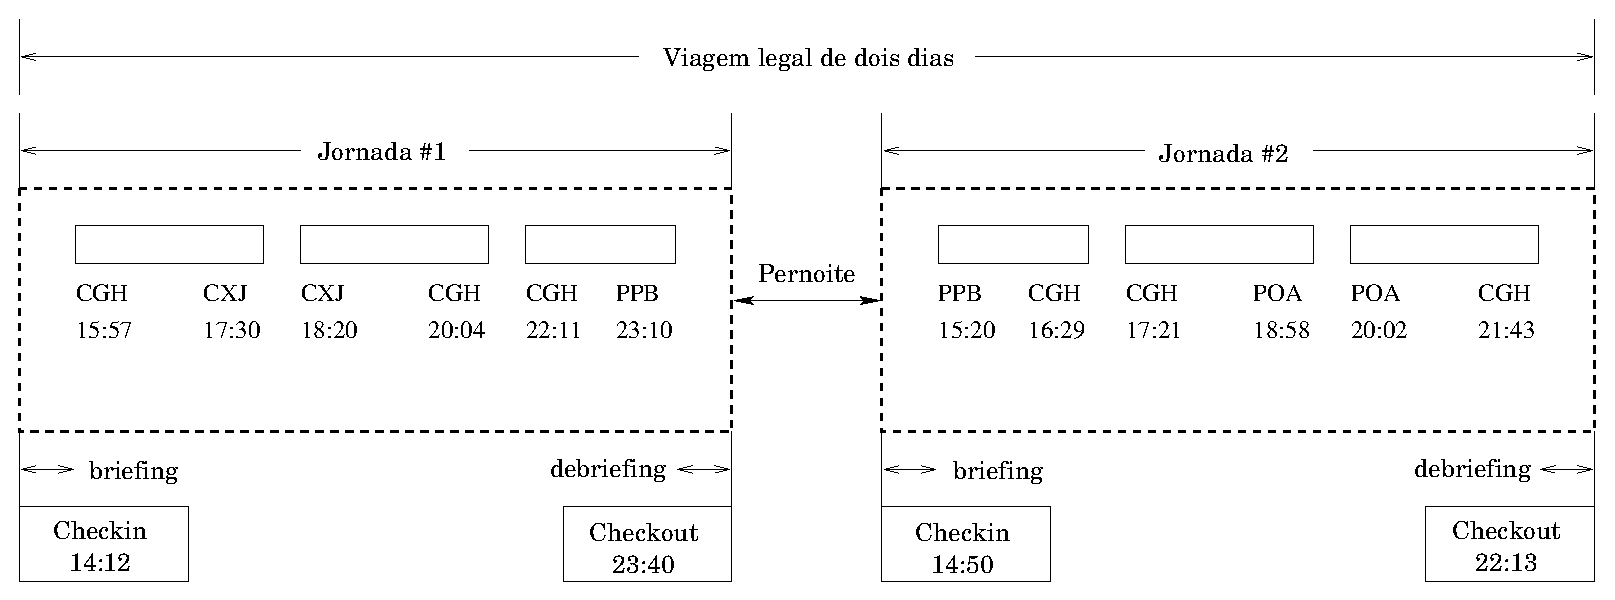
\includegraphics[scale=0.5]{fig/viagem.eps}
		\caption{Exemplo de uma viagem de dois dias para a base CGH.}
		\label{fig:viagem}
	\end{center}
\end{figure}

A Figura~\ref{fig:escala} apresenta o exemplo de uma escala de um determinado tripulante baseado em
GRU. O horizonte de tempo considerado é de 15 dias. Para fins de ilustração, foram alocadas as
viagens (c), (a) e (b) do exemplo anterior nos dias 3, 5--8 e 12--14, respectivamente. Os demais
dias foram preenchidos com períodos de folgas, sobreaviso, reserva e um curso.

\begin{figure}[htbp]
	\begin{center}
		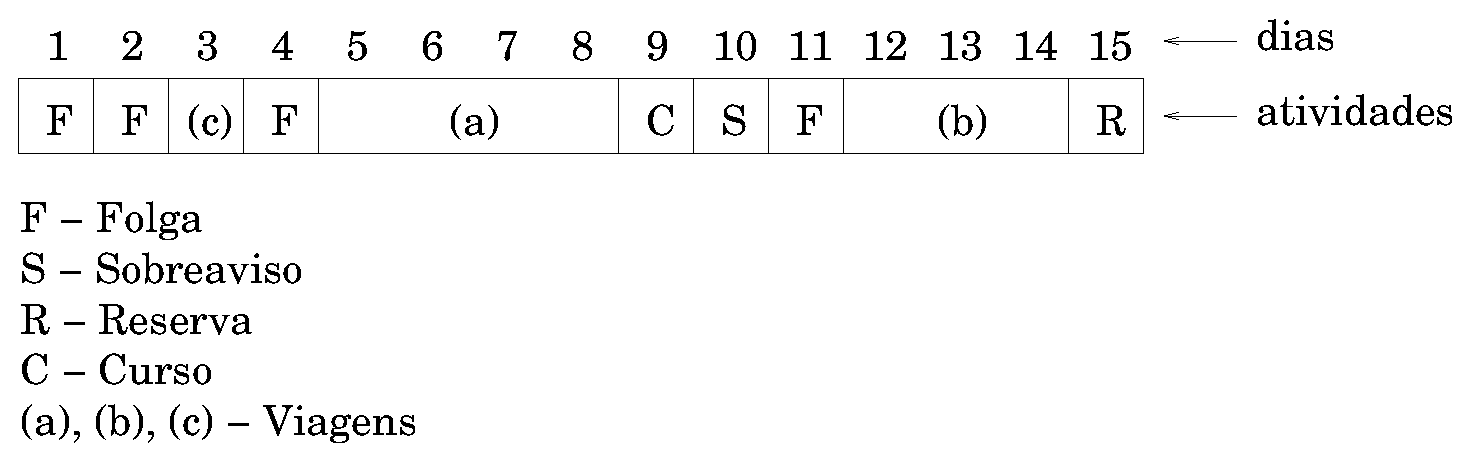
\includegraphics[scale=0.5]{fig/escala.eps}
		\caption{Exemplo de uma escala com diversas atividades para um tripulante baseado em GRU. As 
		viagens (a), (b) e (c) correspondem àquelas mostradas na figura anterior.}
		\label{fig:escala}
	\end{center}
\end{figure}

%%%%%%%%%%%%%%%%%%%%%%%%%%%%%%%%%%%%%%%%%%%%%%%%%%%%%%%%%%%%%%%%%%%%%%%%%%%%%%%%%%%%%%%%%%%%%%%%%%%%

\zerar
\section{Formulação do Problema}
\label{sec:formulacao}

Normalmente o problema do escalonamento de tripulantes é dividido em dois subproblemas que são
resolvidos de forma independente e sequencial. O primeiro deles é conhecido como \emph{problema da
determinação de viagens} (PDV), que consiste na obtenção de um subconjunto de viagens, obedecendo as
regras de trabalho impostas pela legislação, com custo mínimo, cobrindo todas os segmentos de voo
exatamente uma vez. Obtida a solução das viagens, um segundo problema é resolvido, conhecido como
\emph{problema da determinação de escalas} (PDE), cujo objetivo é construir as escalas dos
tripulantes, distribuindo as viagens de tal forma que cada viagem seja atribuída exatamente uma vez
para cada tripulante requerido. Na atribuição, visa-se minimizar os custos e garantir distribuição
uniforme de trabalho. A atribuição das viagens também está sujeita a uma série restrições
reguladoras.

Tanto o PDV quanto o PDE têm sido extensamente estudados na literatura~\cite{gopalakrishnan05}. Em
especial, o primeiro deles recebeu mais atenção, principalmente no contexto norte-americado, dada o
seu potencial em produzir economia significativa de custos. No problema da determinação de escalas,
além de minimizar custos, é importante também levar em conta aspectos da qualidade de vida dos
tripulantes. Uma visão geral e esquemática dos dois problemas é apresentada na
Figura~\ref{fig:escalonamento}.

As modelagens matemáticas usuais do PDV e do PDE são semelhantes e baseiam-se em um problema de 
programação linear inteiro conhecido como \emph{particionamento de um conjunto}. A técnica 
de resolução comum utilizada pode ser descrita como ``gerar-e-otimizar''. Outras abordagens vem 
sendo recentemente propostas, buscando por soluções através de métodos meta-heurísticos. Nas 
próximas seções apresentaremos mais detalhes sobre as duas abordagens.

\begin{figure}[htbp]
	\begin{center}
		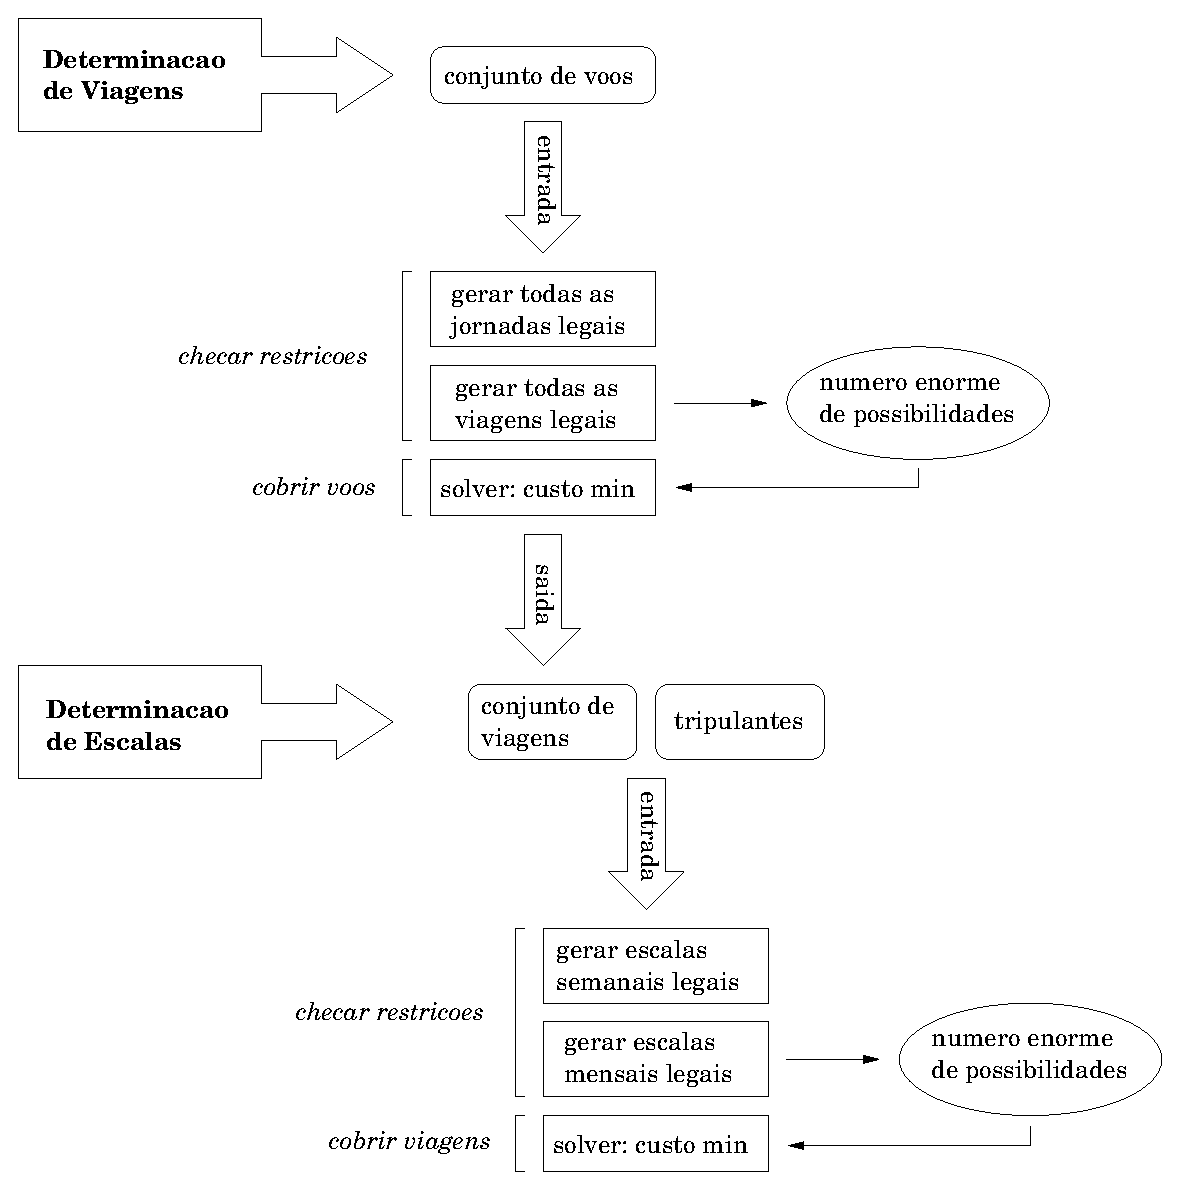
\includegraphics[scale=0.6]{fig/escalonamento.eps}
		\caption{Subproblemas enfrentados na solução do problema de escalonamento de tripulantes 
		(adaptado de~\cite{souai09}).}
		\label{fig:escalonamento}
	\end{center}
\end{figure}

\subsection{Regras de Trabalho e Estrutura de Custo}
\label{sec:regras_e_custos}

Antes de entrarmos nos detalhes sobre a formulação do PDV e do PDE, é interessante explicitar os 
tipos de restrições e a estrutura de custo envolvidos nos problemas, em especial no contexto 
brasileiro, já que há uma diferença significativa com relação aos contextos norte-americano e 
europeu, normalmente empregados nos trabalhos da literatura.

No caso do PDV, a geração de uma viagem é regida por uma série de regras impostas pela Agência
Nacional de Aviação Civil (ANAC), além de restrições impostas por leis trabalhistas e acordos
contratuais. Uma viagem é dita legal se ela obedecer todas as regras impostas pela legislação em
questão. Abaixo apresenta-se valores típicos para as regras que regem a construção de uma viagem em
uma empresa de aviação regular do Brasil com voos de curto e médio alcance:

\begin{itemize}
	\item Duração máxima de uma jornada de trabalho: 11 horas;
	\item Número máximo de horas de voo em uma jornada: 9 horas e 30 minutos;
	\item Número máximo de pousos em uma jornada: 6 pousos;
	\item Descanso mínimo entre jornadas: 12 horas;
	\item Tamanho máximo de uma viagem: 6 dias;
	\item Tempo mínimo de conexão: 30 minutos;
	\item Tempo máximo de conexão: 4 horas;
	\item Número máximo de trocas de aeronave em uma jornada: 2 trocas;
	\item Tempo de briefing: 30 minutos fora de base e 45 minutos dentro;
	\item Tempo de debriefing: 30 minutos.
\end{itemize}

O custo de uma viagem está associado à produtividade mais os custos referentes à estadia do 
tripulante quando esse precisar pernoitar fora da base, além das diárias de alimentação. Uma 
expressão para calcular o custo $c_p$ de uma viagem $p$ é dada por
%
\begin{equation} \label{eq:custov}
	c_p = \sum_{d \in D_p} c_d \, , \;\;
	c_d = \alpha_0 \left[t_d - \left(tp_d - \sum_{i \in I_d} t_i\right)\right] + cp_d \ev
\end{equation}
%
onde
%
\begin{itemize}
	\item[$D_p$:] conjunto de jornadas que constituem a viagem $p$;
	\item[$c_d$:] custo da jornada $d$;
	\item[$\alpha_0$:] custo da hora de trabalho do tripulante;
	\item[$t_d$:] duração da jornada $d$ (em horas);	
	\item[$tp_d$:] tempo de preparação (briefing mais debriefing) usado na jornada $d$;
	\item[$I_d$:] conjunto de etapas que compõem a jornada $d$;
	\item[$t_i$:] duração da etapa $i$, incluindo o tempo mínimo de conexão;
	\item[$cp_d$:] custo do pernoite mais diárias de alimentação da jornada $d$.
\end{itemize}
%
Note que a expressão multiplicando $\alpha$ em (\ref{eq:custov}) representa o tempo que o tripulante
passou trabalhando sem estar voando, portanto representa uma medida de produtividade. Quanto mais
cara a viagem, menor foi a produtividade do tripulante.

No PDE também aplica-se uma série de regras trabalhistas para geração de uma escala legal. Dentre 
elas, podemos citar como mais importantes:

\begin{itemize}
	\item Número mínimo de folgas: 8 folgas, sendo no mínimo 2 em um final de semana;
	\item Intervalo máximo de trabalho sem folgas: 6 dias;
	\item Número máximo de horas de voo em um mês: 85 horas;
	\item Número máximo de horas de uma reserva: 6 horas;
	\item Número máximo de sobreavisos: 2 semanais e 8 mensais.
\end{itemize}

O custo associado a uma dada escala legal montada para um tripulante é bastante dependente da
política de pagamento da empresa. No Brasil, em geral, as companhias costumam pagar um salário fixo
e mais um excedente se o número de horas voadas pelo tripulante extrapolar um determinado valor.
Além disso, horas voadas no período noturno e em domingos e feriados, chamadas horas especiais, são
pagas diretamente a partir do zero. Assim, podemos calcular o custo $c_k$ de uma escala atribuída 
a um tripulante $k$ como
%
\begin{equation}
c_k = \alpha_1 + \alpha_2 \sum_{p \in P_k} e_p 
	+ \alpha_3 \max\left\{0, \left(\sum_{p \in P_k} t_p\right) - mg\right\}
	+ \sum_{p \in P_k} c_p \ev
\end{equation}
%
onde
%
\begin{itemize}
	\item[$\alpha_1$:] remuneração fixa do tripulante;
	\item[$\alpha_2$:] remuneração por cada hora especial realizada;
	\item[$\alpha_3$:] remuneração por cada hora de voo excedente à garantia mínima;
	\item[$P_k$:] conjunto de viagens atribuídas ao tripulante $k$;	
	\item[$e_p$:] horas de voo especiais na viagem $p$;
	\item[$t_p$:] horas de voo na viagem $p$;
	\item[$mg$:] garantia mínima de horas de voo;
	\item[$c_p$:] custo da viagem $p$.
\end{itemize}
%
Note que consideramos apenas a atribuição de viagens na escala de tripulantes. Atividades de reserva
e sobreaviso também entram na remuneração contando como se fossem horas de voo. No caso do
sobreaviso, o valor deve ser multiplicado por $1/3$.

\subsection{Problema da Determinação das Viagens}
\label{sec:viagens}

No problema da determinação das viagens, tem-se como entrada o conjunto de voos a ser operado pela
empresa, o conjunto de bases contratuais dos tripulantes, as regras de trabalho que ditam a
construção de viagens legais e a estrutura de custo como descrita na equação (\ref{eq:custov}). A
saída então deve ser um conjunto de viagens que cubra todos os voos operados exatamente e uma vez e
que gere o custo mínimo (veja Figura~\ref{fig:pdv}).

\begin{figure}[htbp]
	\begin{center}
		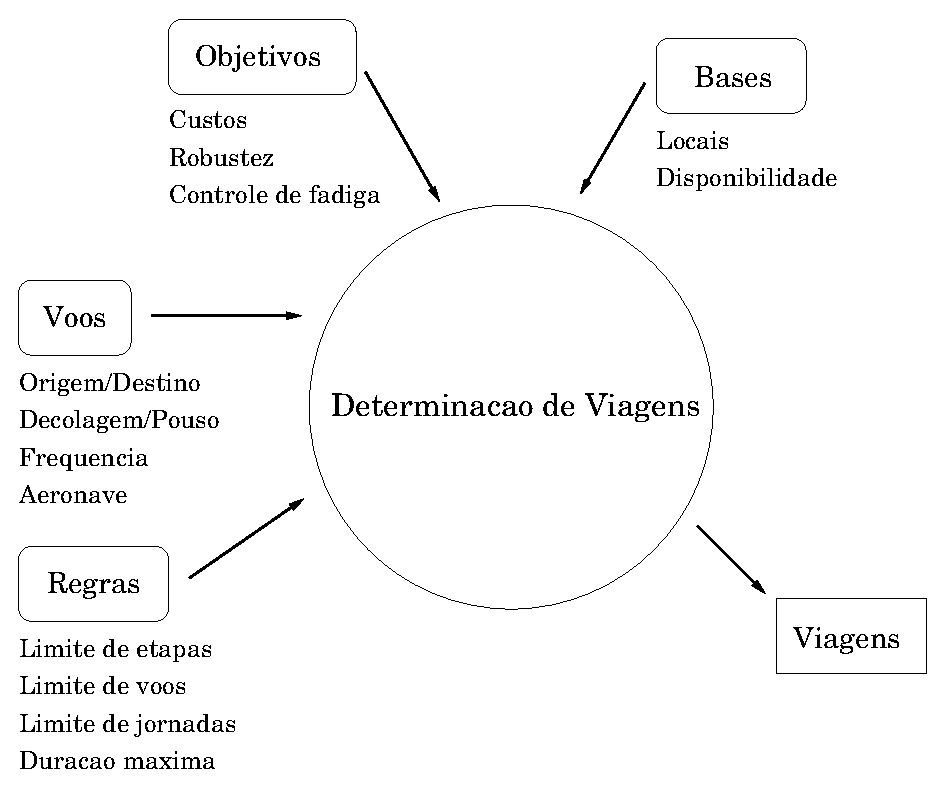
\includegraphics[scale=0.5]{fig/pdv.eps}
		\caption{Representação do problema da determinação de viagens (PDV).}
		\label{fig:pdv}
	\end{center}
\end{figure}

Normalmente os voos das companhias aéreas apresentam uma frequência regular de oferecimento, sendo
que a maioria deles operam diariamente. Outros são oferecidos apenas em alguns dias fixos da semana
e poucos são oferecidos vez ou outra no mês. Costuma-se então inicialmente resolver o problema
diário, onde se assume que todos os voos são repetidos diariamente. Note que para o problema diário,
viagens de vários dias com etapas repetidas são inviáveis. Um segmento de voo repetido causaria o
efeito de mais de uma tripulação ser atribuída para realização dessa etapa, uma vez que quando se
faz a implementação da solução diária, uma tripulação distinta é atribuída a cada um dos dias da
viagem.

O problema semanal é mais complicado porque envolve um maior número de etapas consideradas. De
qualquer forma, a solução do problema semanal pode ser obtido a partir de um ajuste da solução do
problema diário, sem perda significativa de custo~\cite{gopalakrishnan05}. A solução do problema
mensal completo segue da solução do problema semanal. Como a maior parte da redução de custos está
associada à resolução do problema diário, ele se torna o mais importante. Daqui em diante trataremos
apenas do problema diário.

Uma outra simplificação do problema está no fato que os tripulantes são habilitados para operar
apenas um tipo, ou família, de aeronaves dentro de uma frota. Assim, fatora-se o problema da
determinação das viagens por tipo de aeronave. Para cada tipo, resolve-se um PDV considerando apenas
as etapas operadas por aquele tipo. As viagens assim geradas são atribuídas aos tripulantes
habilitados no tipo ao se resolver o PDE.

Há uma formulação natural para o PDV em termos de um problema de programação linear. Suponha que
seja possível gerar e enumerar todas as $n$ viagens associadas a uma dada entrada do problema
contendo $m$ etapas a serem cobertas. Seja $x_j \in \{0, 1\}$ uma variável de decisão que assume o
valor 1 se a viagem $j$ for escolhida na solução de custo mínimo e 0 caso contrário. Então, o PDV
pode ser modelado da seguinte forma:
%
\begin{equation} \label{eq:sppv}
	\begin{array}{rl}
		\text{minimizar} & \displaystyle \sum_{j=1}^n c_j x_j \\
		\text{sujeito à} & \displaystyle \sum_{j=1}^n a_{ij} x_j = 1 \, , \;\; i = 1, \ldots, m \ep \\
	\end{array}
\end{equation}
%
Os coeficientes $a_{ij}$ são definidos por
%
\begin{equation*}
	a_{ij} = \left\{
	\begin{array}{ll}
			1 \ev & \text{se a viagem $j$ cobre a etapa $i$} \\
			0 \ev & \text{caso contrário}
	\end{array}
	\right.
\end{equation*}

As restrições em (\ref{eq:sppv}) garantem que cada etapa seja coberta exatamente uma vez por alguma
viagem. Existe ainda uma formulação alternativa onde as restrições são dadas por
%
\begin{equation} \label{eq:dh}
	\sum_{j=1}^n a_{ij} x_j \geq 1 \, , \;\; i = 1, \ldots, m \ep
\end{equation}
%
Nesse caso uma mesma etapa pode ser coberta por mais de uma viagem e o problema se torna um de
\emph{recobrimento do conjunto}. Do ponto de vista do escalonamento, se uma etapa é coberta por mais
de uma viagem, então uma tripulação estará trabalhando nessa etapa e as demais viajando de
passageiro (situação conhecida por \emph{deadheading}). As vezes essa formulação é necessária para
que se garanta viabilidade da solução. Se o preço a se pagar pela operação com \emph{deadheading} 
for essencialmente o mesmo de uma operação normal, então não há alteração significativa no custo 
da viagem associada. Isso permite que o problema seja modelado com as restrições (\ref{eq:dh}) 
sem alterar a estrutura de custos.

É comum a inserção de restrições adicionais ao modelo que garantem uma distribuição de trabalho
entre as bases compatível com os recursos disponíveis em cada base. Se o número total de bases do
problema considerado é $r$, então as \emph{restrições de bases} são expressas por
%
\begin{equation} \label{eq:bases}
	H_k^L \leq \sum_{j=1}^n h_{kj} x_j \leq H_k^U \, , \;\; k = 1, \ldots, r \ev
\end{equation} 
%
onde $H_k^L$ é o número mínimo de horas disponíveis na base $k$ e $H_k^U$ é seu número máximo. 
Note que $H_k^L$ pode ser diferente de zero desde que se exija que não mais do que um certo número 
de tripulantes fiquem de reserva. O coeficiente $h_{kj}$ dá o número de horas necessárias para 
efetuar a viagem $j$ ($h_{kj} = 0$ se a viagem $j$ não pertencer à base $k$).

O grande problema com a formulação (\ref{eq:sppv}) está no enorme número de variáveis geradas mesmo
nos casos das instâncias pequenas (poucas etapas diárias). A Tabela~\ref{tab:viagens} ilustra o
número de viagens legais geradas, com duração máxima de 3 ou 4 dias, para diversas frotas de
aeronaves. O número enorme de variáveis está associada com a natureza combinatória do problema. A
maioria das empresas aéreas operam em aeroportos conhecidos como \emph{hubs}, onde um grande número
de aeronaves chegam e partem em um mesmo intervalo de tempo, possibilitando que os passageiros
efetuem suas conexões para uma grande quantidade de destinos em pouco tempo. Esse tipo de estrutura
em rede leva à explosão no número de viagens legais que podem ser construídas~\cite{graves93}.
Note da Tabela~\ref{tab:viagens} que apesar do número de viagens ser gigantesco, o número de 
jornadas tem um valor muito mais gerenciável.

\begin{table}[ht]
	\begin{center}
		\begin{tabular}{|c||c|c|c|c|c|}
			\hline
			{\bf Frota} & {\bf Max Dias} & {\bf Etapas} & {\bf Bases} & {\bf Jornadas} & 
			{\bf Viagens} ($\times 10^6$) \\
			\hline
			AAS80 & 3 & 1.152 & 12 & 690.000 & 48.400 \\
			\hline
			AA757 & 3 & 251 & 15 & 7.000 & 1 \\
			\hline
			AA727 & 3 & 375 & 11 & 31.000 & 36 \\
			\hline
			AAF10 & 4 & 307 & 3 & 55.000 & 63.200 \\
			\hline 
			UA737 & 4 & 773 & 7 & 568.000 & 100.000.000 \\
			\hline
			USDC9 & 4 & 478 & 4 & 562.000 & 105.000.000 \\
			\hline
		\end{tabular}
		\caption{Jornadas e viagens legais geradas para um conjunto de frotas de aeronaves de companhias
		norte-americanas (fonte:~\cite{anbil98}).}
		\label{tab:viagens}
	\end{center}
\end{table}

Como o problema de partição é do tipo NP-difícil, a aplicação de métodos diretos de 
otimização é impraticável para qualquer situação real. Os métodos de solução normalmente envolvem
algum tipo de heurística e/ou algum critério de parada que leva a soluções sub-ótimas. Discutiremos
alguns desses métodos na Seção~\ref{sec:metodos}. 

\subsubsection{Gerador de Viagens}
\label{sec:gerador_viagens}

O primeiro passo em direção à solução do PDV consiste na implementação de um gerador de viagens 
eficiente que seja capaz de produzir um grande número de viagens legais em pouco tempo. Como já
mencionamos, os métodos de resolução de (\ref{eq:sppv}) baseiam-se no conceito de 
``gerar-e-otimizar'', e já que as rotinas de otimização estão normalmente prontas em pacotes 
fechados, a parte de geração é de grande importância.

Uma viagem pode ser vista como um caminho especial em um grafo estruturado. Esse grafo é chamado de
\emph{rede de voos} e será detalhado a seguir. 

As etapas na rede de voos podem ser representadas como nós ou arcos. Escolhemos a representação em
termos de arcos. Os nós da rede representam as saídas e chegadas de cada etapa, bem como uma fonte
$s$ e um sorvedouro $t$. Existe um arco representando cada etapa da malha de voos. Para o problema
diário, replicamos cada arco quantas vezes for o número máximo de dias permitido em um viagem. O
conjunto de arcos será denotado por $\calA$.

O nó fonte é ligado ao nó de saída de cada etapa que se origina em uma base específica. O nó de
chegada de cada etapa que termina nessa base é ligado ao sorvedouro. Existem ainda arcos
representando conexões legais entre etapas. Um par de etapas terá um arco de conexão entre eles se
o aeroporto de chegada do primeiro corresponder ao aeroporto de saída do segundo, e o intervalo de
tempo entre a chegada e a saída estiver for uma conexão legal de uma jornada, 
ou descanso regular entre jornadas. 

É fácil notar que toda viagem legal é representada por um caminho $s-t$ na rede de voos. Porém,
existem caminhos $s-t$ que não representam viagens legais pois podem desrespeitar alguma regra de
trabalho, embora as conexões possíveis sejam legais. A estrutura da rede garante que não seja feita
nenhuma conexão entre duas etapas que não tenham suas respectivos destino e origem coincidentes no
espaço e no tempo. Entretanto, não garante, por exemplo, que o número máximo de horas de voo
permitido em uma jornada seja excedido. 

O gerador de viagens funciona aplicando um algoritmo de busca em profundidade à rede de voos. O
algoritmo inicia-se no nó de origem $s$ e explora todas a conexões viáveis $(i, j) \in \calA$, até
retroceder. O processo de busca em profundidade controla a viabilidade das viagens, levando em conta
a duração máxima das jornadas e limites de horas de voo e de pousos.

\subsubsection{Exemplo}
\label{sec:exemplo}

A tabela abaixo mostra um conjunto fictício de 7 etapas operadas diariamente entre as localidades A,
B, C e D. O exemplo é adaptado de~\cite{barnhart03}. 

\begin{table}[ht]
	\begin{center}
		\begin{tabular}{ccccc}
			{\bf \# Etapa} & {\bf Origem} & {\bf Destino} & {\bf Saída} & {\bf Chegada} \\ \hline
			1 & A & B & 08:00 & 09:00 \\
			2 & B & C & 10:00 & 11:00 \\
			3 & C & D & 13:00 & 14:00 \\
			4 & C & A & 15:00 & 16:00 \\
			5 & D & A & 15:00 & 16:00 \\
			6 & A & B & 17:00 & 18:00 \\
			7 & B & C & 11:00 & 12:00 \\
		\end{tabular}
	\end{center}
\end{table}

A rede de voos (parcial) para uma base contratual A é ilustrado na Figura~\ref{fig:rede}, onde são
apresentadas algumas das conexões legais possíveis para clareza do desenho. O caminho vermelho
na figura representa uma viagem legal com dois dias de duração. 

A partir da rede apresentada, montamos as seguintes jornadas válidas (os números representam os
números das etapas)
%
\begin{eqnarray*}
	&& D_1 = \{1\} \ev \hsp D_2 = \{2\} \ev \hsp D_3 = \{3\} \ev \hsp D_4 = \{4\} \\
	&& D_5 = \{5\} \ev \hsp D_6 = \{6\} \ev \hsp D_7 = \{7\} \ev \hsp D_8 = \{1, 2\} \\
	&& D_9 = \{1, 7 ,3\} \ev \hsp D_{10} = \{2, 3\} \ep 
\end{eqnarray*}

Assumindo que as localidades A, B e D sejam bases contratuais, geramos seis viagens, que podem ser
expressas em termos das jornadas como 
%
\begin{eqnarray*}
	&& P_1 = \{D_4, D_8\} \ev \hsp P_2 = \{D_9, D_5\} \ev \hsp P_3 = \{D_5, D_6, D_{10}\} \\
	&& P_4 = \{D_4, D_6, D_7\} \ev \hsp P_5 = \{D_1, D_7, D_4\} \ev \hsp P_6 = \{D_5, D_7, D_9\} \ep 
\end{eqnarray*}

Note que a viagem $P_6$ cobre a etapa $7$ duas vezes, então ela não é válida e deve ser 
desconsiderada. Supondo que os custos associados as viagens sejam $c_1 = c_2 = c_3 = c_4 = 4$ e
$c_5 = 5$, a partir de (\ref{eq:sppv}) obtemos o seguinte problema ($x_i \in \{0, 1\}$, 
$i=1, \ldots, 5$):
%
\begin{equation*}
	\begin{array}{lllllllllllll}
		\text{min} & 4x_1 & + & 4x_2 & + & 4x_3 & + & 4x_4 & + & 5 x_5 & & & \vsp \\ 
		& x_1 & + & x_2 & & & & & + & x_5 & = & 1 & \text{(etapa 1)} \vsp \\
		& x_1 & & & + & x_3 & & & & & = & 1 & \text{(etapa 2)} \vsp \\
		& & & x_2 & + & x_3 & & & & & = & 1 & \text{(etapa 3)} \vsp \\
		& x_1 & & & & & + & x_4 & + & x_5 & = & 1 & \text{(etapa 4)} \vsp \\
		& & & x_2 & + & x_3 & & & & & = & 1 & \text{(etapa 5)} \vsp \\
		& & & & & x_3 & + & x_4 & & & = & 1 & \text{(etapa 6)} \vsp \\
		& & & x_2 & & & + & x_4 & + & x_5 & = & 1 & \text{(etapa 7)}
	\end{array}
\end{equation*}

Se for requerido que pelo menos 3 horas e no máximo 6 horas estejam 
disponíveis nas bases A e D, e no máximo 5 horas na base C, então as restrições de bases
(\ref{eq:bases}) são
%
\begin{equation*}
	\begin{array}{ll}
		3 \leq 4 x_2 + 3 x_5 \leq 6 & \text{(base A)} \vsp \\
		0 \leq 3 x_1 + 3 x_4 \leq 5 & \text{(base C)} \vsp \\
		3 \leq 4 x_3 \leq 6 & \text{(base D)}
	\end{array}
\end{equation*}

A solução ótima para o problema formulado usa as viagens 3 e 5 ($x_3 = x_5 = 1$, 
$x_1 = x_2 = x_4 =  0$) e tem um custo total igual à 9. Por se tratar de um problema pequeno, a
resolução do mesmo pode ser obtido por qualquer pacote de otimização linear.

\begin{figure}[htbp]
	\begin{center}
		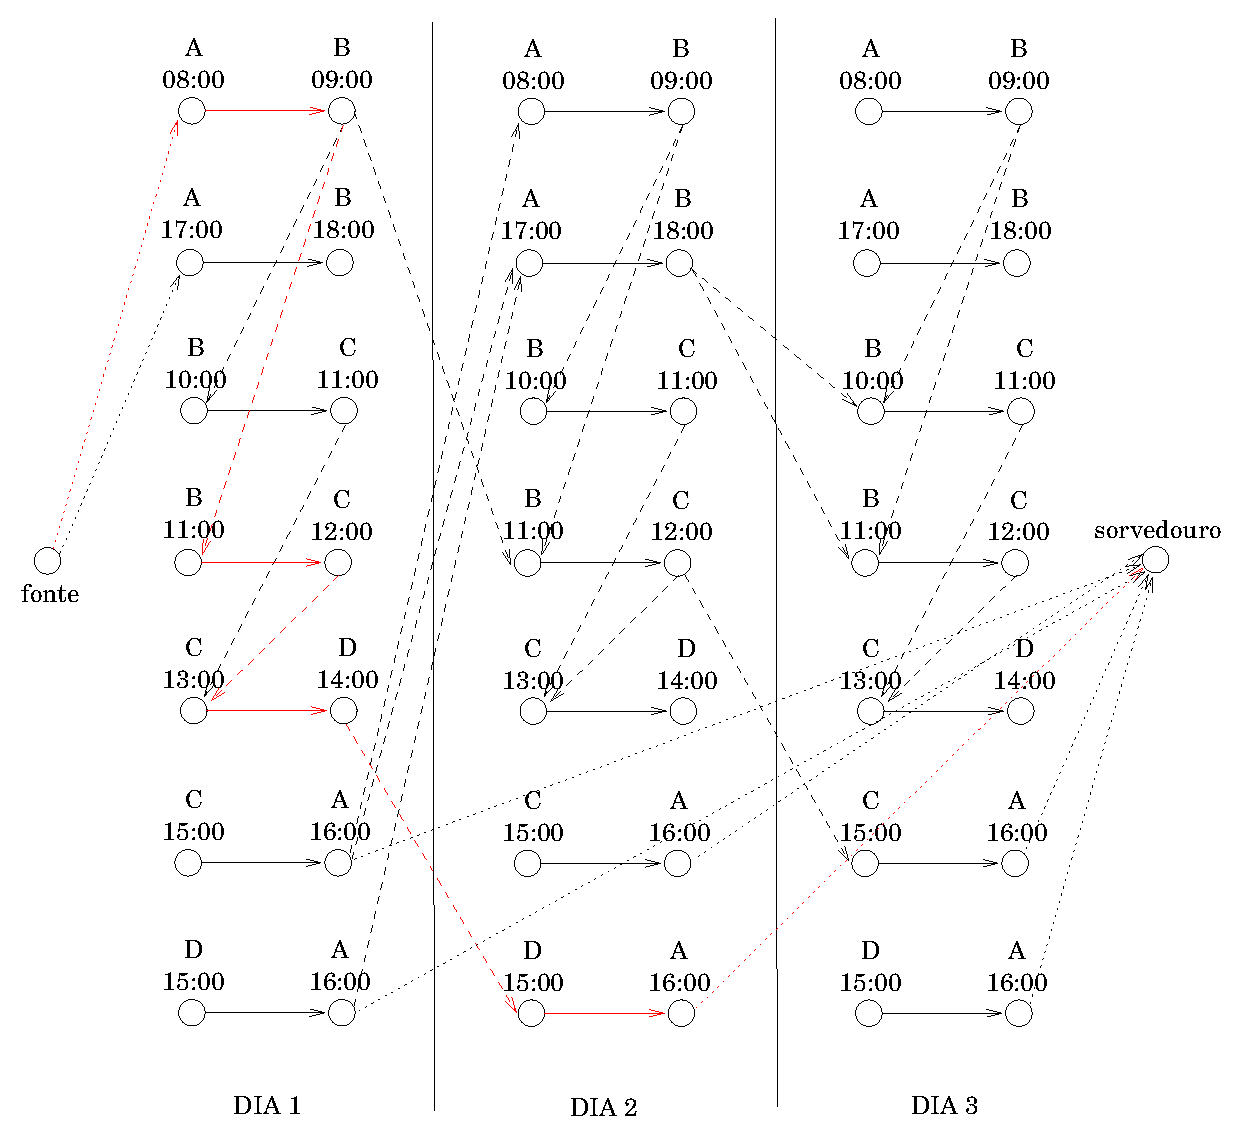
\includegraphics[scale=0.65]{fig/rede.eps}
		\caption{Rede de voos para a base de tripulantes A. Arcos tracejados representam conexões legais
		entre etapas. O caminho em vermelho representa uma das viagens possíveis.}
		\label{fig:rede}
	\end{center}
\end{figure}

\subsection{Problema da Determinação de Escalas}
\label{sec:escalas}

No problema da determinação de escalas (ou, de forma mais restrita, problema da atribuição de
viagens), tem-se como entrada o conjunto de viagens obtido na resolução do PDV na etapa anterior, um
conjunto de atividades extra-voo, as regras utilizadas para confecção de escalas legais e,
finalmente, o conjunto de tripulantes para o qual se deseja gerar as escalas. A saída será uma
escala legal obtida para cada tripulante do conjunto considerado, tal que todas as atividades sejam
atribuídas o número de vezes necessário, e tal que o custo total da solução seja minimizado. Uma
esquema para entrada e saída do problema é apresentado na Figura~\ref{fig:pde}. Uma descrição 
detalhada sobre o problema pode ser encontrada em~\cite{kohl04}.

\begin{figure}[htbp]
	\begin{center}
		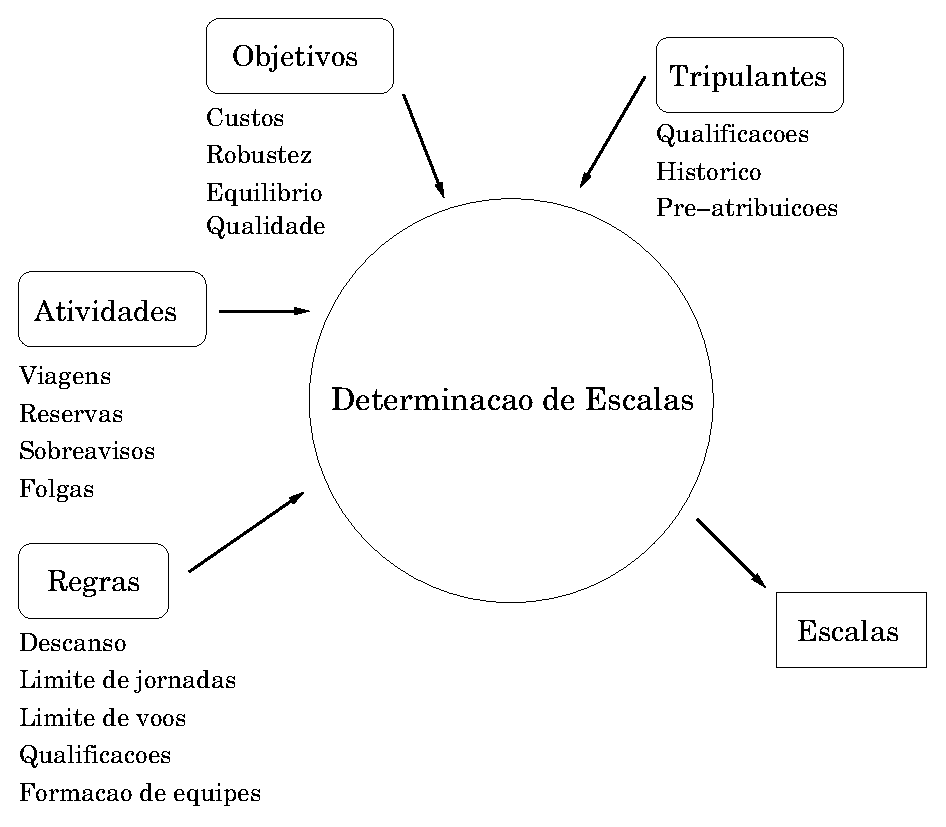
\includegraphics[scale=0.5]{fig/pde.eps}
		\caption{Representação do problema da determinação de escalas (PDE). Adaptado de~\cite{kohl04}.} 
		\label{fig:pde}
	\end{center}
\end{figure}

Nos dados de entrada são fornecidos os registros pessoais de cada tripulante, que incluem suas
qualificações, atividades pré-atribuídas, férias, etc. As qualificações contém informações, por
exemplo, sobre os equipamentos nos quais o tripulante está habilitado, ou sobre destinos onde ele
não pode operar devido a alguma restrição operacional. Atividades pré-atribuídas podem ser
folgas pedidas, exames médico, cursos, etc. Os registros de um tripulante também incluem atributos
acumulados, como o total de horas de vôo realizadas durante o ano corrente. Outros dados de
interesse são, por exemplo, datas limites para treinamentos.

Outro conjunto de dados de entrada é formado pelas atividades a serem cobertas, que consiste das
viagens, reservas, sobreavisos, folgas, atividades de treinamento (\eg treinamento em simulador e
cursos) e atividades em solo (\eg exames médico). Normalmente, na formulação mais restrita do
problema, apenas as viagens devem ser atribuídas de forma automatizada e otimizada. Todas as outras
atividades são atribuídas \emph{a priori}, individualmente para cada tripulante em dias
pré-determinados dentro do horizonte de tempo do planejamento.

As regras típicas para construção de uma escala legal incluem limites máximos para horas de vôo
e jornadas de trabalho, número mínimo de folgas, número máximo de dias consecutivos de trabalho, etc 
(confira Seção~\ref{sec:regras_e_custos}). Essas são conhecidas como \emph{regras horizontais} pois
se aplicam a escalas únicas, e não considerem as outras escalas geradas na solução. Outro conjunto 
de regras, conhecidas por \emph{regras verticais}, aplicam-se à solução como um todo. Um exemplo
típico está na atribuição de uma atividade que necessita ser realizada por mais de um membro de uma tripulação com a mesma função. Outros exemplos de regras verticais são casos do tipo 
``deve voar com'', ou ``não deve voar com''.
 
A função objetivo no PDE é muito dependente da política da empresa. Existem basicamente quatro 
tipos de objetivos que podem ser encontrados em um problema desse tipo. Normalmente as empresas
adotam alguma combinação desses objetivos, seja introduzindo uma função objetivo combinada, seja
introduzindo restrições globais para algum deles enquanto otimizando outros. Os objetivos referem-se
a redução de custos reais, robustez da solução, distribuição equilibrada de trabalho e ``qualidade
de vida'' oferecida.

Vamos agora considerar o problema da determinação de escalas em sua forma mais simples. Sejam dados
um conjunto de atividade $\calA$, de cardinalidade $m_\calA$, e um conjunto de tripulantes $\calC$,
de cardinalidade $m_\calC$. Desejamos obter um conjunto de escalas $\calR_k \subset \calA$ para cada
tripulante $k$, $1 \leq k \leq m_\calC$, que particiona $\calA$,
%
\begin{equation*}
	\calA = \calR_1 \cup \calR_2 \cup \cdots \cup \calR_{m_\calC} \ev
\end{equation*}
%
de forma a minimizar alguma função objetivo linear nos custos $c_k$ de cada escala.

Um grande número de escalas $R_j \subset \calA$ podem ser geradas para cada tripulante. Idealmente,
todas as escalas legais poderiam ser geradas, mas para o resultado seria um número enorme dada a 
natureza combinatória do problema. Depois da geração de $n$ escalas, um problema de particionamento 
é resolvido para selecionar a melhor combinação de escalas que minimizem o custo da função objetivo.

Seja $x_j \in \{0, 1\}$, $1 \leq j \leq n$, uma variável de decisão cujo valor é 1 se a escala
$\calR_j$ for escolhida na solução, e 0 caso contrário. Seja $c_j$, $1 \leq j \leq n$, o custo 
associado à escala $\calR_j$. Seja ainda $A$ a matriz $m \times n$, onde $m = m_\calC + m_\calA$, 
com coeficientes $a_{ij}$ definidos por
%
\begin{equation*}
	a_{ij} = \left\{
	\begin{array}{ll}
			1 \ev & \text{se a escala $j$ foi gerada para o tripulante $i$, $i = 1, \ldots, m_\calC$} \\
			1 \ev & \text{se a escala $j$ contém a atividade $i - m_\calC$, 
			$i = m_\calC + 1, \ldots, m$} \\
			0 \ev & \text{caso contrário}
	\end{array}
	\right.
\end{equation*}

Com essas definições, o PDE é formulado da seguinte forma:
%
\begin{equation} \label{eq:sppe}
	\begin{array}{rl}
		\text{minimizar} & \displaystyle \sum_{j=1}^n c_j x_j \\
		\text{sujeito à} & \displaystyle \sum_{j=1}^n a_{ij} x_j = 1 \, , \;\; i = 1, \ldots, m \ep \\
	\end{array}
\end{equation}
%
Note que para cada tripulante exatamente uma escala deve ser determinada e cada atividade deve ser
atribuída a exatamente uma escala.

Suponha, por exemplo, que para cada tripulante três escalas sejam geradas. Então $n = 3m_\calC$, 
e a matriz de restrições $A$ assume forma semelhante~a:

\begin{center}
	\scalebox{0.85} {
		\begin{tabular}{ccccc}
			\begin{tabular}{ccc}
				\hline 
				\multicolumn{3}{c}{Tripulante$_1$} \\ \hline
				$\calR_1$ &	$\calR_2$ & $\calR_3$ \\ \hline
				1 & 1 & 1 \\
				0 & 0 & 0 \\
				$\vdots$ & $\vdots$ & $\vdots$ \\
				0 & 0 & 0 \\
				1 & 1 & 0 \\
				0 & 1 & 1 \\
				$\vdots$ & $\vdots$ & $\vdots$ \\
				1 & 0 & 1
			\end{tabular}
			& 
			\begin{tabular}{ccc}
				\hline 
				\multicolumn{3}{c}{Tripulante$_2$} \\ \hline
				$\calR_4$ &	$\calR_5$ & $\calR_6$ \\ \hline
				0 & 0 & 0 \\
				1 & 1 & 1 \\
				$\vdots$ & $\vdots$ & $\vdots$ \\
				0 & 0 & 0 \\
				1 & 0 & 1 \\
				0 & 0 & 1 \\
				$\vdots$ & $\vdots$ & $\vdots$ \\
				0 & 0 & 0
			\end{tabular}	
			& 
			\hspace{-0.3cm}
			\begin{tabular}{c}
				$\cdots$ \\
				$\cdots$ \\
				$\cdots$ \\
				$\cdots$ \\
				$\ddots$ \\
				$\cdots$ \\
				$\cdots$ \\
				$\cdots$ \\
				$\ddots$ \\
				$\cdots$
			\end{tabular}
			\hspace{-0.3cm}
			& 
			\begin{tabular}{ccc}
				\hline 
				\multicolumn{3}{c}{Tripulante$_{|\calC|}$} \\ \hline
				$\calR_{n-2}$ &	$\calR_{n-1}$ & $\calR_n$ \\ \hline
				0 & 0 & 0 \\
				0 & 0 & 0 \\
				$\vdots$ & $\vdots$ & $\vdots$ \\
				1 & 1 & 1 \\
				0 & 1 & 0 \\
				1 & 0 & 1 \\
				$\vdots$ & $\vdots$ & $\vdots$ \\
				0 & 1 & 0
			\end{tabular}	
			&
			\hspace{-0.3cm}
			\begin{tabular}{ccc}
				& & \\
				& & \\
				= & 1 & Atribuições \\
				= & 1 & \\
				$\vdots$ & $\vdots$ & \\
				= & 1 & \\
				= & 1 & Atividades \\
				= & 1 & \\
				$\vdots$ & $\vdots$ & \\
				= & 1 & 				
			\end{tabular} 
		\end{tabular}
	}
\end{center}

Existem dois tipos de restrições representadas pela matriz $A$ no modelo básico. As \emph{restrições 
de atribuições} garantem que todo tripulante tenha exatamente uma escala atribuída. Elas formam 
o primeiro bloco $m_\calC \times n$ de $A$. As \emph{restrições de atividades} garantem que cada 
atividade será atribuída exatamente uma vez na solução, formando o bloco final $m_\calA \times n$ 
final da matriz $A$.

Assim como no PDV, a formulação exposta acima do PDE apresenta dificuldade de resolução devido ao
número excessivo de variáveis e restrições. Mesmo os otimizadores mais potentes não são capazes de
resolver instâncias práticas do problemas em tempo viável. A solução é utilizar algum tipo de
heurística que encontre uma resposta sub-ótima para o problema, ou técnicas de otimização mais
avançadas como a geração implícita de colunas.

\subsection{Formulação Integrada}
\label{sec:integrado}

Atualmente o PDV e o PDE são eficientemente tratados por uma série de técnicas que garantem soluções
próximas do ótimo com um tempo de processamento aceitável. Sistemas comerciais foram desenvolvidos
em torna dessas técnicas, sendo diariamente utilizados na maioria das empresas para resolução de
seus problemas de escalonamento~\cite{gopalakrishnan05}.

Um problema muito mais complexo seria o da integração entre o PDV e PDE, onde esses dois
sub-problemas seriam analisados e resolvidos simultaneamente. A vantagem dessa abordagem é motivada
pelos fatos descritos a seguir.

Primeiro, a fatoração do problema não permite que se estime adequadamente o custo
real de um escalonamento global. De fato, na determinação das viagens, busca-se minimizar o custo
associado à baixa produtividade de uma jornada de trabalho. Entretanto, o custo real do planejamento
só pode ser calculado após a atribuição das viagens aos tripulantes, ou seja, depois da solução do
PDE. Isso porque, para um dado horizonte de tempo, faz-se o pagamento de um salário fixo e mais 
um valor adicional para as horas excedentes.

Segundo, o conjunto ``ótimo de viagens'' provido na solução do PDV é determinado sem considerar o
número e a disponibilidade dos diferentes tripulantes. É claro que se pode incorporar no modelo as
restrições de bases (\ref{eq:bases}), mas elas fornecem apenas uma estimativa da mão de obra
disponível, pois não consideram as restrições impostas pelas regras que limitam a geração de escalas
legais. Na realidade, a disponibilidade real só é considerada enquanto se resolve o problema da
determinação de escalas.

A tendência recente nos trabalhos sobre escalonamento de tripulantes é de lidar com a versão
integrada do problema~\cite{saddoune12, souai09}, que apontam para ganhos econômicos da ordem de 5\%
com relação a versão sequencial. O problema completo, entretanto, é de difícil resolução, dado a
combinação do número de variáveis que já eram grandes no PDV e no PDE. Reporta-se
em~\cite{saddoune12} longos tempos de processamento mesmo para instâncias pequenas utilizando
técnicas de geração de colunas e agregação dinâmica de restrições. Uma alternativa interessante é a
utilização de meta-heurísticas como o algoritmo genético aplicado em~\cite{souai09}.

%%%%%%%%%%%%%%%%%%%%%%%%%%%%%%%%%%%%%%%%%%%%%%%%%%%%%%%%%%%%%%%%%%%%%%%%%%%%%%%%%%%%%%%%%%%%%%%%%%%%

\zerar
\section{Métodos de Solução}
\label{sec:metodos}

TODO

%%%%%%%%%%%%%%%%%%%%%%%%%%%%%%%%%%%%%%%%%%%%%%%%%%%%%%%%%%%%%%%%%%%%%%%%%%%%%%%%%%%%%%%%%%%%%%%%%%%%

% Bibliografia BiBTeX
\bibliography{../bib/crew_scheduling}
\bibliographystyle{plain}
 
\end{document}

